\documentclass[10pt,a4paper,onecolumn]{article}
\usepackage[utf8]{inputenc}
\usepackage{marginnote}
\usepackage{graphicx}
\usepackage{xcolor}
\usepackage{authblk,etoolbox}
\usepackage{titlesec}
\usepackage{calc}
\usepackage{hyperref}
\hypersetup{breaklinks=true,
            bookmarks=true,
            pdfauthor=
{
      Sophie Bavard,
      Héloïse Théro,
  },
            pdftitle=
{
[Re] Adaptive properties of differential learning rates for positive and
negative outcomes
},
            colorlinks=true,
            citecolor=blue,
            urlcolor=blue,
            linkcolor=blue,
            pdfborder={0 0 0}}
\urlstyle{same}
\usepackage{tcolorbox}
\usepackage{ragged2e}
\usepackage{fontspec}
\usepackage{fontawesome}
\usepackage{caption}
\usepackage{listings}
\lstnewenvironment{code}{\lstset{language=Haskell,basicstyle=\small\ttfamily}}{}



%\usepackage{fancyvrb}
%\VerbatimFootnotes
%\usepackage{graphicx}
%\usepackage{mdframed}
%\newmdenv[backgroundcolor=lightgray]{Shaded}


\usepackage{longtable,booktabs}

\usepackage[
  backend=biber,
%  style=alphabetic,
%  citestyle=numeric
]{biblatex}
\bibliography{bibliography.bib}



% --- Macros ------------------------------------------------------------------
\renewcommand*{\bibfont}{\small \sffamily}

\definecolor{red}{HTML}{CF232B}
\newcommand{\ReScience}{Re{\bfseries \textcolor{red}{Science}}}

\newtcolorbox{rebox}
   {colback=blue!5!white, colframe=blue!40!white,
     boxrule=0.5pt, arc=2pt, fonttitle=\sffamily\scshape\bfseries,
     left=6pt, right=20pt, top=6pt, bottom=6pt}

\newtcolorbox{repobox}
   {colback=red, colframe=red!75!black,
     boxrule=0.5pt, arc=2pt, left=6pt, right=6pt, top=3pt, bottom=3pt}

% fix for pandoc 1.14     
\newcommand{\tightlist}{%
  \setlength{\itemsep}{1pt}\setlength{\parskip}{0pt}\setlength{\parsep}{0pt}}

% --- Style -------------------------------------------------------------------
\renewcommand*{\bibfont}{\small \sffamily}
\renewcommand{\captionfont}{\small\sffamily}
\renewcommand{\captionlabelfont}{\bfseries}

\makeatletter
\renewcommand\@biblabel[1]{{\bf #1.}}
\makeatother

% --- Page layout -------------------------------------------------------------
\usepackage[top=3.5cm, bottom=3cm, right=1.5cm, left=1.5cm,
            headheight=2.2cm, reversemp, includemp, marginparwidth=4.5cm]{geometry}

% --- Section/SubSection/SubSubSection ----------------------------------------
\titleformat{\section}
  {\normalfont\sffamily\Large\bfseries}
  {}{0pt}{}
\titleformat{\subsection}
  {\normalfont\sffamily\large\bfseries}
  {}{0pt}{}
\titleformat{\subsubsection}
  {\normalfont\sffamily\bfseries}
  {}{0pt}{}
\titleformat*{\paragraph}
  {\sffamily\normalsize}


% --- Header / Footer ---------------------------------------------------------
\usepackage{fancyhdr}
\pagestyle{fancy}
%\renewcommand{\headrulewidth}{0.50pt}
\renewcommand{\headrulewidth}{0pt}
\fancyhead[L]{\hspace{-1cm}
\includegraphics[width=4.0cm]{rescience-logo.pdf}}
\fancyhead[C]{}
\fancyhead[R]{} 
\renewcommand{\footrulewidth}{0.25pt}

\fancyfoot[L]{\hypersetup{urlcolor=red}
              \sffamily \ReScience~$\vert$
              \href{http://rescience.github.io}{rescience.github.io}
              \hypersetup{urlcolor=blue}}
\fancyfoot[C]{\sffamily 1 - \thepage}
\fancyfoot[R]{\sffamily Sep 2015 $\vert$
                        Volume \textbf{1} $\vert$
                        Issue \textbf{1}}
\pagestyle{fancy}
\makeatletter
\let\ps@plain\ps@fancy
\fancyheadoffset[L]{4.5cm}
\fancyfootoffset[L]{4.5cm}

% --- Title / Authors ---------------------------------------------------------
% patch \maketitle so that it doesn't center
\patchcmd{\@maketitle}{center}{flushleft}{}{}
\patchcmd{\@maketitle}{center}{flushleft}{}{}
% patch \maketitle so that the font size for the title is normal
\patchcmd{\@maketitle}{\LARGE}{\LARGE\sffamily}{}{}
% patch the patch by authblk so that the author block is flush left
\def\maketitle{{%
  \renewenvironment{tabular}[2][]
    {\begin{flushleft}}
    {\end{flushleft}}
  \AB@maketitle}}
\makeatletter
\renewcommand\AB@affilsepx{ \protect\Affilfont}
%\renewcommand\AB@affilnote[1]{{\bfseries #1}\hspace{2pt}}
\renewcommand\AB@affilnote[1]{{\bfseries #1}\hspace{3pt}}
\makeatother
\renewcommand\Authfont{\sffamily\bfseries}
\renewcommand\Affilfont{\sffamily\small\mdseries}
\setlength{\affilsep}{1em}

\LetLtxMacro{\OldIncludegraphics}{\includegraphics}
\renewcommand{\includegraphics}[2][]{\OldIncludegraphics[width=12cm, #1]{#2}}


% --- Document ----------------------------------------------------------------
\title{[Re] Adaptive properties of differential learning rates for positive and
negative outcomes}

    \usepackage{authblk}
                        \author[1]{Sophie Bavard}
                    \author[1]{Héloïse Théro}
                            \affil[1]{Laboratoire de Neurosciences Cognitives Computationnelles (ENS -
INSERM), Département d'Études Cognitives, École normale supérieure, PSL
Research University, 29 rue d'Ulm, 75005 Paris, France}
            
\date{\vspace{-5mm}
      \sffamily \small \href{mailto:sophie.bavard@gmail.com, thero.heloise@gmail.com}{sophie.bavard@gmail.com, thero.heloise@gmail.com}}


\setlength\LTleft{0pt}
\setlength\LTright{0pt}


\begin{document}
\maketitle

\marginpar{
  %\hrule
  \sffamily\small
  %\vspace{2mm}
  {\bfseries Editor}\\
  Olivia Guest\\

  {\bfseries Reviewers}\\
        Benoît Girard\\
        Xavier Hinault\\
  
  {\bfseries Received}  Feb, 9, 2018\\
  {\bfseries Accepted}  ?, ?, ?\\
  {\bfseries Published} ?, ?, ?\\

  {\bfseries Licence}   \href{http://creativecommons.org/licenses/by/4.0/}{CC-BY}

  \begin{flushleft}
  {\bfseries Competing Interests:}\\
  The authors have declared that no competing interests exist.
  \end{flushleft}

  \hrule
  \vspace{3mm}

  \hypersetup{urlcolor=white}
  
    \vspace{-1mm}
  \begin{repobox}
    \bfseries\normalsize
      \href{http://github.com/rescience/rescience-submission/article}{\faGithubAlt~Article repository}
  \end{repobox}
      \vspace{-1mm}
  \begin{repobox}
    \bfseries\normalsize
      \href{http://github.com/rescience/rescience-submission/code}{\faGithubAlt~Code repository}
  \end{repobox}
        \hypersetup{urlcolor=blue}
}

\begin{rebox}
\sffamily {\bfseries A reference implementation of}
\small
\begin{flushleft}
\begin{itemize}
    \item[→] Cazé, R. D., \& van der Meer, M. A. (2013). Adaptive properties of
differential learning rates for positive and negative outcomes.
Biological cybernetics, 107(6), 711-719.
https://doi.org/10.1007/s00422-013-0571-5
  \end{itemize}\par
\end{flushleft}
\end{rebox}


\hypertarget{introduction}{%
\section{Introduction}\label{introduction}}

Reinforcement learning represents a fundamental cognitive process:
learning by trial and error to maximize rewards and minimize
punishments. Current and most influential theoretical models of
reinforcement learning assume a unique learning rate parameter,
independently of the outcome valence \cite{sutton1998introduction, o2004dissociable, behrens2007learning}. However
human participants were shown to integrate differently positive and
negative outcomes \cite{frank2004carrot, frank2007genetic, sharot2011unrealistic}. This
motivated Cazé and van der Meer to implement a modified version of the
reinforcement learning model, with two distinct learning rates for
positive and negative outcomes \cite{caze2013adaptive}.

They have shown that although differential learning rates shifted reward
predictions and could thus be seen as a maladaptive bias, this model can
outperform the classical reinforcement learning model on tasks with
specific outcome probabilities. Following Cazé and van der Meer's
predictions \cite{caze2013adaptive}, a subsequent empirical article have modeled human behavior
on these specific tasks \cite{gershman2015learning}. The question
is still an active research area, as various articles have further
investigated the difference learning rates bias
\cite{garrett2014robust, moutsiana2015human, shah2016pessimistic, 
garrett2017optimistic, lefebvre2017behavioural, palminteri2017confirmation}.

At the time we first submitted this manuscript, we were not aware that the
 code of the reference article was freely available \href{https://github.com/rcaze/13_02CaVa}{online}. 
Our model and analysis scripts 
were therefore implemented from scratch using Python (version 3.6.3), with 
the NumPy (version 1.14.0) and Matplotlib (version 2.1.1) libraries.

% online (\url{https://github.com/rcaze/13_02CaVa}

\hypertarget{methods}{%
\section{Methods}\label{methods}}

We first implemented our scripts on Matlab, as we were more familiar
with this language, and then adapted them on Python.

We used the modeling description of the reference article to implement
our replication. They used standard Q-learners with a softmax action
selection rule \cite{sutton1998introduction}, and their precise
description enabled us to implement them with low difficulty. But we
found four ambiguities in the simulation procedure.

First, the authors described their analytical results to be valid for
``\(Q_0 \neq \{-1, 1\}\)'' in section 2, but did not specify what value
of \(Q_0\) they used in all the following simulations. We chose to use
\(Q_0 = 0\), as this initial value is the middle point between the two
possible outcomes (i.e., -1 and 1). As we replicated all the original
figures, even the dynamics in the beginning of the learning curves (see
Figures ~\ref{fig:figure2}A, ~\ref{fig:figure3} and ~\ref{fig:figure4}B),
we believe the reference article must have used similar initial
Q-values.

Second, regarding the parameter setting for Figure ~\ref{fig:figure1}'s
simulations, the ratio of \(\alpha^+\) over \(\alpha^-\) was said to be
either 0.25, 1 or 4, but they did not specify what were the exact values
of \(\alpha^+\) and \(\alpha^-\) used. We thus set them according to the
following description of the pessimistic, rational and optimistic agents
in section 3, i.e.:

\begin{itemize}
\tightlist
\item
  \(\alpha^+ = 0.1\) and \(\alpha^- = 0.4\) for the ratio of 0.25
\item
  \(\alpha^+ = 0.1\) and \(\alpha^- = 0.1\) for the ratio of 1
\item
  \(\alpha^+ = 0.4\) and \(\alpha^- = 0.1\) for the ratio of 4
\end{itemize}

Third, the number of iterations made to generate Figures
 \ref{fig:figure3} and \ref{fig:figure4} were not indicated, and we
assumed the authors used the same number as in Figures
 \ref{fig:figure1} and \ref{fig:figure2} (i.e., 5,000 runs).

Finally, it was unclear in the reference article whether the performances 
were averaged based on the probabilities to select the correct action, 
or based on the proportion of correct choices. We define the proportion 
of correct choices as the number of trials in which the correct action 
was chosen divided by the total number of trials. In contrast, the 
probability to select the correct action is computed by the model 
on each trial, and then used to choose an action. For example
Figure \ref{fig:figure2}'s legend indicated: ``Mean probability of choosing the best
arm'', suggesting that the probabilities themselves were used. However,
when commenting the figure in section 3, the authors appeared to say
that the actual choices were rather used: ``the optimistic agent learns
to take the best action significantly more than the rational agent''.
For our analyses, we started by using the probabilities of choice, as
this would lead to more clear, less noise-corrupted results. However we
then obtained very smooth learning curves, and were unable to reproduce
the spikiness of the original Figures \ref{fig:figure2}, 
\ref{fig:figure3} and \ref{fig:figure4}. We thus computed the
proportions of implemented choices for all our figures.

\hypertarget{results}{%
\section{Results}\label{results}}

All our figures reproduced the patterns of the original results. We were
even able to replicate the fine-grained details of the learning curves,
like the early bumps in performance in the high-reward task (Figures
 \ref{fig:figure2}A, \ref{fig:figure3} and \ref{fig:figure4}B, right
panels, around 50-100 trials). In Figure \ref{fig:figure1}, the mean
and the variance of the Q-values were also very similar as the ones in
the original figure. We numbered our figures in the same way as the reference article. 

The only discrepancy we found was in Figure \ref{fig:figure4}A.
Although the general pattern was replicated, our learning curves
appeared smoother than in the reference article. As the number of
simulations were not explicitly specified for this figure, we cannot
know if this is due to us running a higher number of simulations than
the reference article, or from another difference in model
implementation. However, we obtained similar noise when dividing 
the number of simulations by ten, suggesting the original authors 
used around 500 iterations for this part of the figure.

\hypertarget{fig:figure1}{%
\begin{figure}
\centering
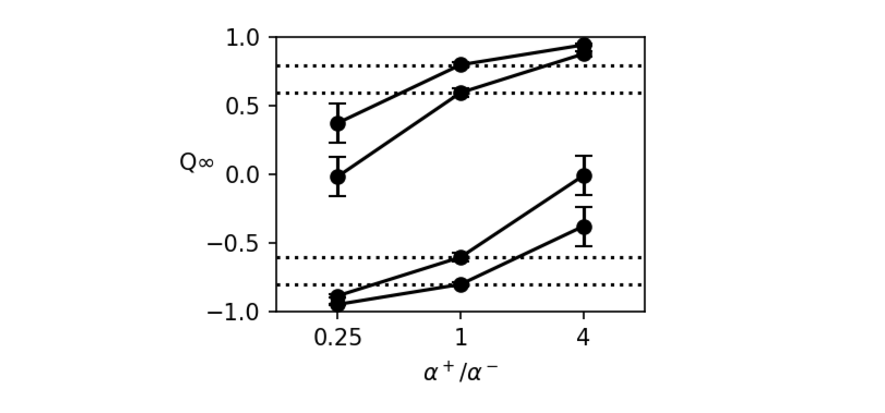
\includegraphics{Figure1.pdf}
\caption{Average estimated Q-values after 800 trials averaged for
different ratios of \(\alpha^+\) and \(\alpha^-\). The dotted lines
represent the underlying average reward: 0.8, 0.6, -0.6, -0.8. The error
bars represent the variance of the estimated
Q-values.}\label{fig:figure1}
\end{figure}
}

\hypertarget{fig:figure2}{%
\begin{figure}
\centering
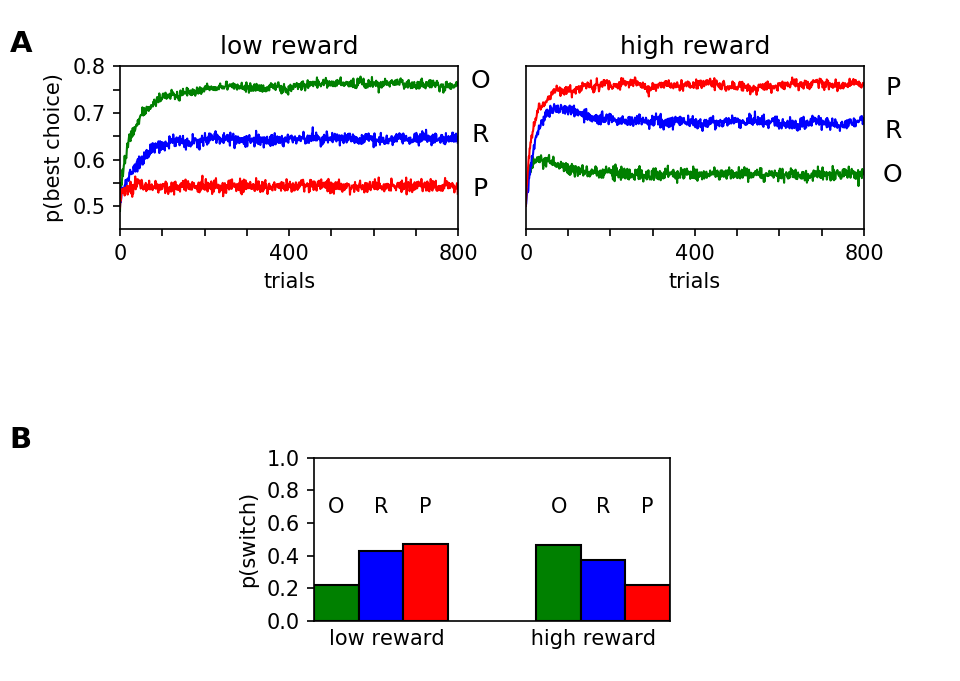
\includegraphics{Figure2.png}
\caption{\textbf{A.} Performance, i.e., proportion of choices for the
best action, for the three agents: Rational (R, \(\alpha^+=\alpha^-\),
blue line), Optimistic (O, \(\alpha^+>\alpha^-\), green line) and
Pessimistic (P, \(\alpha^+<\alpha^-\), red line). In this figure and the
following ones, the left (resp. right) panel corresponds to the
low-reward (resp. high-reward) task. \textbf{B.} Proportion of action
switch after 800 trials for each agent, in the two different
tasks.}\label{fig:figure2}
\end{figure}
}

\hypertarget{fig:figure3}{%
\begin{figure}
\centering
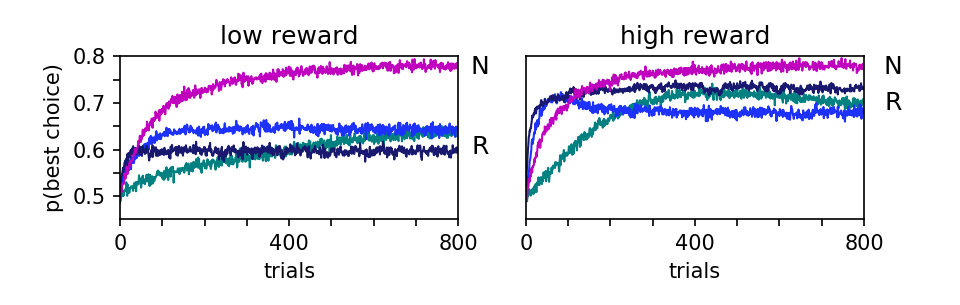
\includegraphics{Figure3.png}
\caption{The performances of the Meta-learner (N) are shown in
\emph{purple} and those of the Rational agents (R) in different colors
of blue (in \emph{teal} for \(\alpha = 0.01\), in \emph{royal blue} for
\(\alpha = 0.1\) and in \emph{navy blue} for
\(\alpha = 0.4\)).}\label{fig:figure3}
\end{figure}
}

\hypertarget{fig:figure4}{%
\begin{figure}
\centering
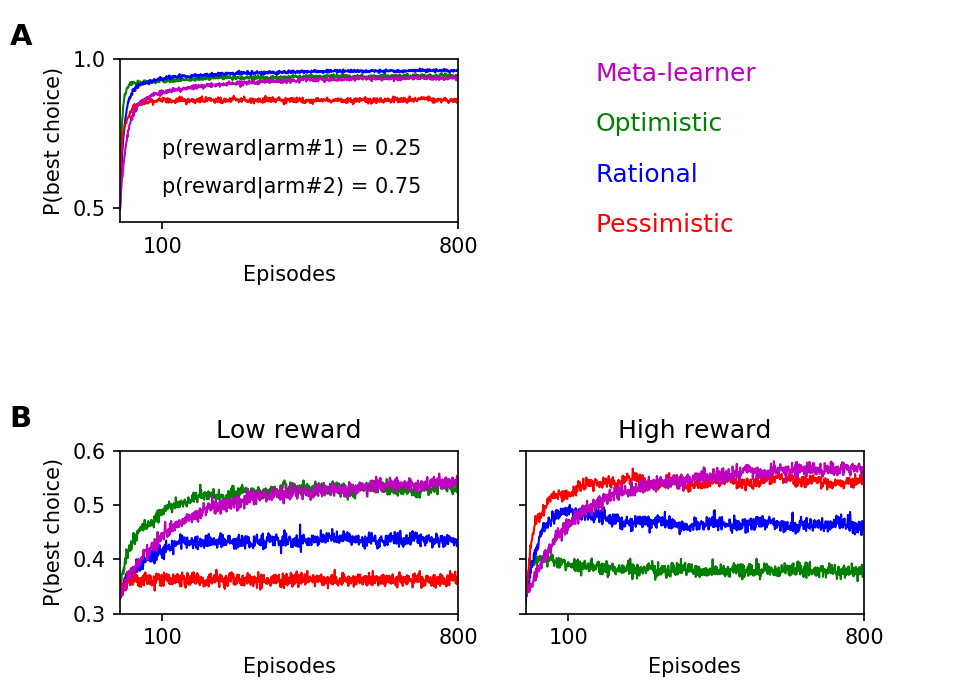
\includegraphics{Figure4.png}
\caption{The performances of the Meta-learner, Optimistic, Rational and
Pessimistic agents \textbf{A.} in a task where the probabilities of
reward are 0.75 and 0.25 for the two choices. \textbf{B.} in a
``three-armed bandit'' task.}\label{fig:figure4}
\end{figure}
}

\hypertarget{conclusion}{%
\section{Conclusion}\label{conclusion}}

All the figures in Cazé and van der Meer \cite{caze2013adaptive} have been successfully
reproduced with high fidelity, and we confirm the validity of their
simulations. Overall the whole replication procedure was smooth: the
models were implemented with low difficulty, and the simulations were
quite straightforward apart from a few obscure details. We hope this
replication can foster future research in the domain.

{\sffamily \small
  \printbibliography[title=References]
}
\end{document}
